% ==========================================================================
%  WW3 Runtime Optimisation — Beamer Presentation
%  Author : Lenny Hucher (MET Norway)
%  Date   : 27 May 2026
%
%  Compile with:
%    pdflatex presentation.tex   (twice for ToC / navigation)
%
%  Theme: metropolis (texlive-beamer or texlive-full).
%  Fallback: comment \usetheme{metropolis} and uncomment the two lines below.
% ==========================================================================

\documentclass[aspectratio=169,10pt]{beamer}

\usetheme{metropolis}
% \usetheme{default}
% \usecolortheme{seahorse}

% --------------------------------------------------------------------------
% Packages
% --------------------------------------------------------------------------
\usepackage{graphicx}
\usepackage{tikz}
\usetikzlibrary{positioning, arrows.meta, shapes.geometric,
                fit, backgrounds, calc, decorations.pathreplacing}
\usepackage{pgfplots}
\pgfplotsset{compat=1.18}
\usepackage{booktabs}
\usepackage{xcolor}
\usepackage{amsmath}
\usepackage{amssymb}
\usepackage{bm}
\usepackage{listings}
\usepackage{multicol}

% --------------------------------------------------------------------------
% Colours
% --------------------------------------------------------------------------
\definecolor{metnb}{RGB}{0,71,145}       % MET Norway blue
\definecolor{metnlb}{RGB}{210,230,250}   % light blue fill
\definecolor{w3org}{RGB}{214,95,14}      % WW3 orange
\definecolor{w3grn}{RGB}{40,150,80}      % WW3 green
\definecolor{w3red}{RGB}{200,30,30}      % warning red
\definecolor{w3lgr}{RGB}{240,240,240}    % light grey

% metropolis accent colour (overrides default)
\setbeamercolor{alerted text}{fg=w3org}
\setbeamercolor{example text}{fg=w3grn}

% --------------------------------------------------------------------------
% Listings (bash snippets)
% --------------------------------------------------------------------------
\lstset{
  basicstyle   = \ttfamily\scriptsize,
  keywordstyle = \color{metnb}\bfseries,
  commentstyle = \color{w3grn}\itshape,
  stringstyle  = \color{w3org},
  backgroundcolor = \color{metnlb!40},
  frame        = single,
  framerule    = 0.5pt,
  rulecolor    = \color{metnb!40},
  breaklines   = true,
  numbers      = none,
}

% --------------------------------------------------------------------------
% Helper tikz styles
% --------------------------------------------------------------------------
\tikzset{
  rankbox/.style  = {draw=metnb!70, fill=metnlb, rounded corners=2pt,
                     minimum width=1.1cm, minimum height=0.85cm,
                     align=center, font=\tiny},
  ompbox/.style   = {draw=w3grn!70, fill=w3grn!20, rounded corners=2pt,
                     minimum width=0.9cm, minimum height=1.1cm,
                     align=center, font=\tiny},
  asyncbox/.style = {draw=w3org!70, fill=w3org!20, rounded corners=2pt,
                     minimum width=2.1cm, minimum height=0.5cm,
                     align=center, font=\tiny},
  phasebox/.style = {draw=metnb!70, fill=metnlb, rounded corners=3pt,
                     minimum width=3.6cm, minimum height=0.7cm,
                     align=center, font=\scriptsize\bfseries},
  leverbox/.style = {draw=metnb!60, fill=metnlb, rounded corners=4pt,
                     minimum width=3.3cm, minimum height=0.8cm,
                     align=center, font=\small\bfseries},
  jobarr/.style   = {->, thick, metnb},
  jobbox/.style   = {draw=metnb!70, fill=metnlb, rounded corners=3pt,
                     minimum width=2.5cm, minimum height=1.0cm,
                     align=center, font=\small},
}

% --------------------------------------------------------------------------
% Metadata
% --------------------------------------------------------------------------
\title{Optimising WaveWatch III on HPC}
\subtitle{A systematic benchmarking study — from 417\,s to 290\,s}
\author{Lenny Hucher}
\institute{PhD student, MET Norway}
\date{27 May 2026}
\titlegraphic{
\includegraphics[height=0.8cm]{met-rgb-horisontal-eng.jpg}}

% ==========================================================================
\begin{document}
% ==========================================================================

\maketitle

% ==========================================================================
\section{How WW3 works}
% ==========================================================================

% ------------------------------------------------------------------
\begin{frame}{CARRA2 configuration}

  \textbf{Discretisation used in this study:}
  \begin{columns}[T]
    \begin{column}{0.48\textwidth}
      \textbf{Spatial grid:}
      \begin{itemize}
        \item $2869\!\times\!2869$ curvilinear (CURV)
        \item $\approx\!4.2$\,M active sea points
        \item Domain: Arctic + North Atlantic
      \end{itemize}

      \vspace{0.5em}
      \textbf{Spectral discretisation:}
      \begin{itemize}
        \item $N_k = 32$ frequencies
        \item $N_\theta = 36$ directions
        \item $\Rightarrow$ \textbf{NSPEC = 1152 bins}
      \end{itemize}
    \end{column}
    \begin{column}{0.48\textwidth}
      \textbf{Time stepping:}
      \begin{itemize}
        \item Global timestep $\Delta t_{\max} = 270$\,s
        \item Propagation substep $\Delta t_{xy} = 90$\,s
        \item Source term integration: implicit
      \end{itemize}

      \vspace{0.5em}
      \textbf{Physics:}
      \begin{itemize}
        \item Wind input + dissipation: ST4
        \item Non-linear interactions: NL1 (DIA)
        \item Bottom friction: BT4
        \item Ice: IC0 (off) --- IC1--IC4 to be tested
      \end{itemize}
    \end{column}
  \end{columns}
\end{frame}

% ------------------------------------------------------------------
\begin{frame}[shrink=5]{The inner compute loop}

  Each global timestep ($\Delta t_{\max} = 270$\,s) WW3 performs:

  \vspace{0.6em}
  \begin{center}
  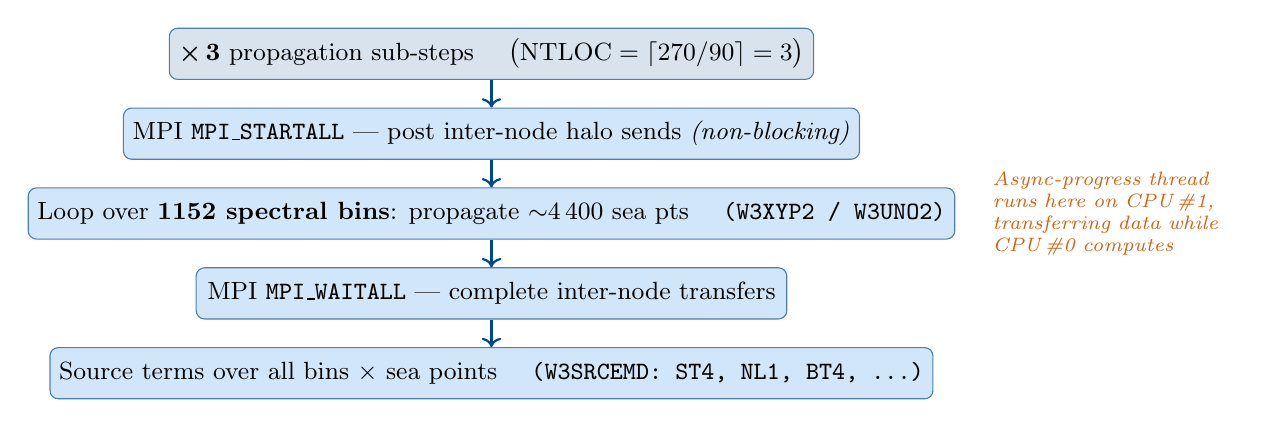
\begin{tikzpicture}[
    node distance = 0.4cm,
    box/.style = {draw=metnb!70, fill=metnlb, rounded corners=3pt,
                  minimum width=7.5cm, minimum height=0.65cm,
                  align=center, font=\small},
    arr/.style = {->, thick, metnb},
  ]
    \node[box, fill=metnb!15] (spec)
      {$\bm{\times}$\,\textbf{3} propagation sub-steps
       \quad $\bigl(\mathrm{NTLOC} = \lceil 270/90 \rceil = 3\bigr)$};
    \node[box, below=0.35cm of spec] (halo1)
      {MPI \texttt{MPI\_STARTALL} --- post inter-node halo sends \emph{(non-blocking)}};
    \node[box, below=0.35cm of halo1] (prop)
      {Loop over \textbf{1152 spectral bins}: propagate $\sim$4\,400 sea pts
       \quad \texttt{(W3XYP2 / W3UNO2)}};
    \node[box, below=0.35cm of prop] (wait)
      {MPI \texttt{MPI\_WAITALL} --- complete inter-node transfers};
    \node[box, below=0.35cm of wait] (src)
      {Source terms over all bins $\times$ sea points
       \quad \texttt{(W3SRCEMD: ST4, NL1, BT4, \ldots)}};
    \draw[arr] (spec)  -- (halo1);
    \draw[arr] (halo1) -- (prop);
    \draw[arr] (prop)  -- (wait);
    \draw[arr] (wait)  -- (src);
    % side note
    \node[right=0.35cm of prop, font=\scriptsize, color=w3org,
          text width=3cm, align=left]
      {\textit{Async-progress thread runs here on CPU\,\#1, transferring data while CPU\,\#0 computes}};
  \end{tikzpicture}
  \end{center}
\end{frame}

% ------------------------------------------------------------------
\begin{frame}[shrink=8]{Domain decomposition --- MPI}

  \begin{columns}[T]
    \begin{column}{0.52\textwidth}
      \textbf{Spatial decomposition:}
      \begin{itemize}
        \item $\sim$4.2\,M sea points split across MPI ranks
        \item Each rank owns a \emph{contiguous patch} of sea points
              ($\sim$4\,400 pts/rank at 960 ranks)
        \item Every rank loops over \textbf{all 1152 spectral bins}
              independently
        \item After each propagation sub-step: halo exchange with
              spatial neighbours
      \end{itemize}

      \vspace{0.6em}
      \textbf{Production layout (Fahrenheit):}
      \begin{center}
        \begin{tabular}{lr}
          \toprule
          Nodes & 16 \\
          MPI ranks/node & 60 \\
          Total MPI ranks & 960 \\
          CPUs/rank & 2 \\
          Total CPUs allocated & 1\,920 \\
          \bottomrule
        \end{tabular}
      \end{center}
    \end{column}

    \begin{column}{0.44\textwidth}
      \begin{center}
      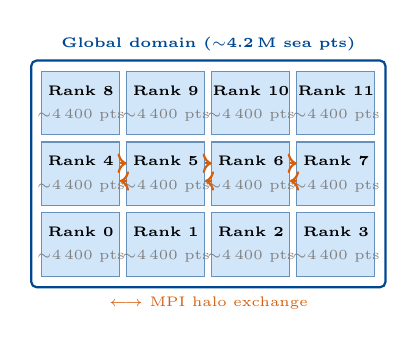
\begin{tikzpicture}[scale=0.9]
        % Global domain boundary
        \draw[thick, metnb, rounded corners=2pt]
          (-0.1,-0.1) rectangle (4.9,3.1);
        \node[above, font=\tiny\bfseries, color=metnb] at (2.4,3.1)
          {Global domain ($\sim$4.2\,M sea pts)};

        % 4 × 3 rank tiles
        \foreach \i in {0,1,2,3}{
          \foreach \j in {0,1,2}{
            \pgfmathtruncatemacro{\r}{\i + \j*4}
            \draw[fill=metnlb, draw=metnb!60]
              ({0.05 + \i*1.2}, {0.05 + \j*1.0})
              rectangle ({0.05 + \i*1.2 + 1.1}, {0.05 + \j*1.0 + 0.9});
            \node[font=\tiny\bfseries] at ({0.05+\i*1.2+0.55},{0.05+\j*1.0+0.63})
              {Rank \r};
            \node[font=\tiny, color=gray] at ({0.05+\i*1.2+0.55},{0.05+\j*1.0+0.28})
              {\raisebox{0pt}{$\sim$}4\,400 pts};
          }
        }
        % halo exchange arrows (horizontal, middle row)
        \foreach \i in {0,1,2}{
          \draw[->, w3org, thick]
            ({0.05+\i*1.2+1.1},{0.05+1.0+0.6}) --
            ({0.05+\i*1.2+1.2},{0.05+1.0+0.6});
          \draw[->, w3org, thick]
            ({0.05+\i*1.2+1.2},{0.05+1.0+0.35}) --
            ({0.05+\i*1.2+1.1},{0.05+1.0+0.35});
        }
        \node[below, font=\tiny, color=w3org] at (2.4,-0.1)
          {$\longleftrightarrow$ MPI halo exchange};
      \end{tikzpicture}
      \end{center}
    \end{column}
  \end{columns}
\end{frame}

% ------------------------------------------------------------------
\begin{frame}[shrink=10]{Parallelism modes in WW3}

  \begin{columns}[T,onlytextwidth]

    % --- MPI-only ---
    \begin{column}{0.33\textwidth}
      \begin{center}
        {\small\bfseries\color{metnb} MPI-only (current default)}
      \end{center}
      \begin{center}
      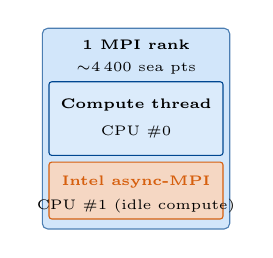
\begin{tikzpicture}[scale=0.85]
        \draw[draw=metnb!70, fill=metnlb, rounded corners=2pt]
          (0,0) rectangle (2.8,3.0);
        \node[font=\tiny\bfseries] at (1.4,2.75) {1 MPI rank};
        \node[font=\tiny] at (1.4,2.4) {$\sim$4\,400 sea pts};
        % compute box
        \draw[draw=metnb, fill=metnlb!80, rounded corners=1pt]
          (0.1,1.1) rectangle (2.7,2.2);
        \node[font=\tiny\bfseries] at (1.4,1.85) {Compute thread};
        \node[font=\tiny] at (1.4,1.45) {CPU \#0};
        % async box
        \draw[draw=w3org, fill=w3org!25, rounded corners=1pt]
          (0.1,0.15) rectangle (2.7,1.0);
        \node[font=\tiny\bfseries, color=w3org] at (1.4,0.7) {Intel async-MPI};
        \node[font=\tiny] at (1.4,0.35) {CPU \#1 (idle compute)};
      \end{tikzpicture}
      \end{center}
      \vspace{2pt}
      \scriptsize
      Sequential over spectral bins.\\
      CPU\,\#1 reserved for MPI progress;\\
      compute runs on CPU\,\#0 only.
    \end{column}

    % --- OMPH ---
    \begin{column}{0.33\textwidth}
      \begin{center}
        {\small\bfseries\color{w3grn} OMPH — hybrid (spatial)}
      \end{center}
      \begin{center}
      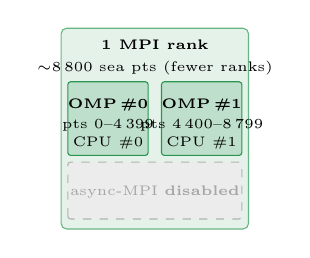
\begin{tikzpicture}[scale=0.85]
        \draw[draw=w3grn!70, fill=w3grn!12, rounded corners=2pt]
          (0,0) rectangle (2.8,3.0);
        \node[font=\tiny\bfseries] at (1.4,2.75) {1 MPI rank};
        \node[font=\tiny] at (1.4,2.4) {$\sim$8\,800 sea pts (fewer ranks)};
        % OMP thread 0
        \draw[draw=w3grn, fill=w3grn!30, rounded corners=1pt]
          (0.1,1.1) rectangle (1.3,2.2);
        \node[font=\tiny\bfseries] at (0.7,1.85) {OMP\,\#0};
        \node[font=\tiny] at (0.7,1.55) {pts 0--4\,399};
        \node[font=\tiny] at (0.7,1.28) {CPU \#0};
        % OMP thread 1
        \draw[draw=w3grn, fill=w3grn!30, rounded corners=1pt]
          (1.5,1.1) rectangle (2.7,2.2);
        \node[font=\tiny\bfseries] at (2.1,1.85) {OMP\,\#1};
        \node[font=\tiny] at (2.1,1.55) {pts 4\,400--8\,799};
        \node[font=\tiny] at (2.1,1.28) {CPU \#1};
        % async off
        \draw[draw=gray!60, fill=gray!15, rounded corners=1pt, dashed]
          (0.1,0.15) rectangle (2.7,1.0);
        \node[font=\tiny, color=gray!70] at (1.4,0.55) {async-MPI \textbf{disabled}};
      \end{tikzpicture}
      \end{center}
      \vspace{2pt}
      \scriptsize
      \texttt{W3XYP2} inner sea-point\\
      loop threaded with OpenMP.\\
      Both CPUs do compute work.
    \end{column}

    % --- OMPG ---
    \begin{column}{0.33\textwidth}
      \begin{center}
        {\small\bfseries\color{gray!70} OMPG — hybrid (spectral)}
      \end{center}
      \begin{center}
      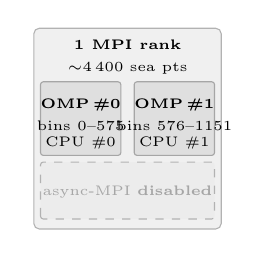
\begin{tikzpicture}[scale=0.85]
        \draw[draw=gray!60, fill=gray!12, rounded corners=2pt]
          (0,0) rectangle (2.8,3.0);
        \node[font=\tiny\bfseries] at (1.4,2.75) {1 MPI rank};
        \node[font=\tiny] at (1.4,2.4) {$\sim$4\,400 sea pts};
        % OMP thread 0 — spectral bins 0-575
        \draw[draw=gray!70, fill=gray!25, rounded corners=1pt]
          (0.1,1.1) rectangle (1.3,2.2);
        \node[font=\tiny\bfseries] at (0.7,1.85) {OMP\,\#0};
        \node[font=\tiny] at (0.7,1.55) {bins 0--575};
        \node[font=\tiny] at (0.7,1.28) {CPU \#0};
        % OMP thread 1 — spectral bins 576-1151
        \draw[draw=gray!70, fill=gray!25, rounded corners=1pt]
          (1.5,1.1) rectangle (2.7,2.2);
        \node[font=\tiny\bfseries] at (2.1,1.85) {OMP\,\#1};
        \node[font=\tiny] at (2.1,1.55) {bins 576--1151};
        \node[font=\tiny] at (2.1,1.28) {CPU \#1};
        \draw[draw=gray!60, fill=gray!15, rounded corners=1pt, dashed]
          (0.1,0.15) rectangle (2.7,1.0);
        \node[font=\tiny, color=gray!70] at (1.4,0.55) {async-MPI \textbf{disabled}};
      \end{tikzpicture}
      \end{center}
      \vspace{2pt}
      \scriptsize
      Source-term loop over spectral\\
      bins threaded with OpenMP.\\
      Compatible with OMPH.
    \end{column}

  \end{columns}

  \vspace{0.5em}
  \begin{block}{Key setting for hybrid configs}
    \centering\small
    \texttt{I\_MPI\_ASYNC\_PROGRESS=0} \quad+\quad \texttt{OMP\_NUM\_THREADS=2}
  \end{block}
\end{frame}

% ==========================================================================
\section{WW3 and the HPC system}
% ==========================================================================

% ------------------------------------------------------------------
\begin{frame}[shrink=10]{How WW3 interacts with HPC}

  A production WW3 run is a \textbf{chain of three Slurm jobs}:

  \vspace{0.3em}
  \begin{center}
  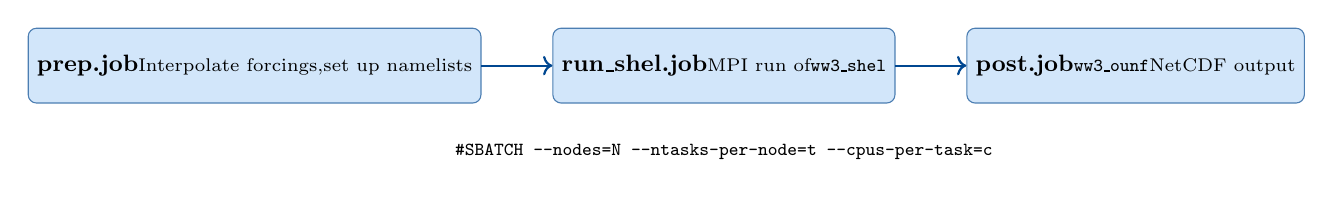
\begin{tikzpicture}[node distance=0.9cm, scale=0.95, every node/.style={scale=0.95}]
    \node[jobbox] (prep)
      {\textbf{prep.job}\newline{\scriptsize Interpolate forcings,\newline set up namelists}};
    \node[jobbox, right=0.9cm of prep] (shel)
      {\textbf{run\_shel.job}\newline{\scriptsize MPI run of\newline\texttt{ww3\_shel}}};
    \node[jobbox, right=0.9cm of shel] (post)
      {\textbf{post.job}\newline{\scriptsize \texttt{ww3\_ounf}\newline NetCDF output}};
    \draw[jobarr] (prep) -- (shel);
    \draw[jobarr] (shel) -- (post);
    % Below: parameters
    \node[below=0.4cm of shel, font=\scriptsize, align=center]
      {\texttt{\#SBATCH --nodes=N --ntasks-per-node=t --cpus-per-task=c}};
  \end{tikzpicture}
  \end{center}

  \vspace{0.2em}
  \begin{columns}[T]
    \begin{column}{0.48\textwidth}
      \textbf{Why} \texttt{cpus-per-task $\geq$ 2}\textbf{?}\\[3pt]
      Without a second CPU, Intel MPI's async-progress thread shares CPU\,\#0
      with the compute thread $\Rightarrow$ \texttt{MPI\_WaitAll} blocks
      $\Rightarrow$ roughly $\times$2 slowdown.
    \end{column}
    \begin{column}{0.48\textwidth}
      \textbf{What is ``async-progress''?}\\[3pt]
      A background thread that pumps the OFI network stack while the compute
      thread runs, so \texttt{MPI\_WaitAll} returns immediately.
    \end{column}
  \end{columns}
\end{frame}

% ==========================================================================
\section{How to optimise WW3}
% ==========================================================================

% ------------------------------------------------------------------
\begin{frame}{Seven optimisation levers}

  \begin{columns}[T]
    \begin{column}{0.48\textwidth}
      \textbf{\color{metnb} No recompile needed:}
      \begin{enumerate}
        \item Grid \& timestep
        \item I/O frequency
        \item Output variables
        \item Namelists
        \item[6.] Job layout
      \end{enumerate}

      \vspace{0.5em}
      \small
      Start with these --- they can give 10--30\,\% gains
      without touching the binary.
    \end{column}
    \begin{column}{0.48\textwidth}
      \textbf{\color{w3org} Recompile required:}
      \begin{enumerate}
        \item[5.] Switches (physics, numerics, parallelism)
        \item[7.] Compilation flags
      \end{enumerate}

      \vspace{0.5em}
      \small
      Switches select physics modules and parallelism modes.
      Flags control optimisation level, SIMD, and PGO.
    \end{column}
  \end{columns}

  \vspace{0.8em}
  \centering\small
  Each lever is independent; gains stack but must be measured on the target machine.
\end{frame}

% ------------------------------------------------------------------
\begin{frame}[shrink=10]{Levers 1--3: Grid, I/O, output variables}

  \begin{columns}[T]
    \begin{column}{0.48\textwidth}
      \textbf{Grid \& timestep (lever 1)}
      \begin{itemize}
        \item Coarser resolution $\Rightarrow$ fewer sea points $\Rightarrow$ less compute
        \item Larger $\Delta t_{xy}$ reduces the number of propagation sub-steps
              (CFL must still hold)
        \item Larger $\Delta t_{\max}$ reduces source-term call frequency
      \end{itemize}

      \vspace{0.5em}
      \textbf{I/O frequency (lever 2)}
      \begin{itemize}
        \item WW3 output is \textbf{serial} (one rank writes)
        \item Every output step is a synchronisation barrier
        \item Reduce output frequency when time resolution allows
        \item Same for forcing reads (wind, ice)
      \end{itemize}
    \end{column}
    \begin{column}{0.48\textwidth}
      \textbf{Output variables (lever 3)}
      \begin{itemize}
        \item Spectral output (\texttt{OUNF}) is very expensive ---
              use it only for target points or validation periods
        \item Directional spectra on the full grid: high bandwidth cost
        \item Keep only the fields needed for your analysis
      \end{itemize}

    \end{column}
  \end{columns}
\end{frame}

% ------------------------------------------------------------------
\begin{frame}[fragile,shrink=8]{Lever 4: Namelists}

  Some physics parameters change runtime significantly \emph{without}
  changing the science of interest.

  \vspace{0.4em}
  \begin{exampleblock}{Example: cumulative breaking term (\texttt{\&SDS4})}
\begin{lstlisting}[language={}]
&SDS4
  SDSCUM = 0.0   ! disable cumulative breaking integral
/
\end{lstlisting}
    Setting \texttt{SDSCUM = 0.0} skips an inner integral in the dissipation
    term.  Measured savings: \textbf{5--20\,\%} runtime,
    depending on grid resolution.
  \end{exampleblock}

  \vspace{0.4em}
  \textbf{Other namelist knobs worth checking:}
  \begin{itemize}
    \item Frequency table (number of discrete frequencies) ---
          reducing $N_k$ from 36 to 32 saves $\sim\!10$\,\% source-term time
  \end{itemize}
\end{frame}

% ------------------------------------------------------------------
\begin{frame}[shrink=12]{Lever 5: WW3 switches}

  Switches are set \textbf{at compile time} and select physics, numerics,
  and parallelism.  Changing them requires a rebuild.

  \vspace{0.2em}
  \begin{columns}[T]
    \begin{column}{0.48\textwidth}
      \textbf{Parallelism switches:}
      \begin{itemize}
        \item \texttt{SHRD} --- shared memory, single process
        \item \texttt{DIST} + \texttt{MPI} --- distributed memory (standard)
        \item \texttt{OMPH} --- OpenMP over \textbf{sea points}
        \item \texttt{OMPG} --- OpenMP over \textbf{spectral bins}
      \end{itemize}

      \vspace{0.2em}
      \textbf{Numerics switches:}
      \begin{itemize}
        \item \texttt{PR0}/\texttt{PR1}/\texttt{PR2}/\texttt{PR3} ---
              propagation accuracy
        \item \texttt{UNO} --- UNO scheme \quad \texttt{UQ} --- QUICK scheme
      \end{itemize}
    \end{column}
    \begin{column}{0.48\textwidth}
      \textbf{Physics switches:}
      \begin{itemize}
        \item \texttt{ST4} / \texttt{ST6} --- wind-input + dissipation
        \item \texttt{IC0} \ldots \texttt{IC4} ---
              ice source terms (IC0 = off)
        \item \texttt{BT1} / \texttt{BT4} --- bottom friction
        \item \texttt{NL1} / \texttt{NL2} --- non-linear interactions
      \end{itemize}

      \vspace{0.3em}
      \begin{exampleblock}{Performance tips (from colleagues)}
        \small
        \textbf{PR2 + UNO} instead of PR3 + UQ can give \textbf{10--20\,\%} speedup.\\
        \textbf{ST4} scales better and is faster than ST6.
      \end{exampleblock}
    \end{column}
  \end{columns}
\end{frame}

% ------------------------------------------------------------------
\begin{frame}[fragile,shrink=15]{Lever 6: Job script --- layout tuning}

  \begin{columns}[T]
    \begin{column}{0.54\textwidth}
      Three Slurm parameters control total core usage:
      \[
        \underbrace{N}_{\text{nodes}}
        \times
        \underbrace{t}_{\text{tasks/node}}
        \times
        \underbrace{c}_{\text{CPUs/task}}
        = \text{total CPUs}
      \]
\begin{lstlisting}[language={}]
#SBATCH --nodes=16
#SBATCH --ntasks-per-node=60
#SBATCH --cpus-per-task=2
...
export OMP_NUM_THREADS=$SLURM_CPUS_PER_TASK
\end{lstlisting}

      \vspace{0.3em}
      \textbf{Scale-study strategy:}
      \begin{enumerate}\small
        \item Fix $N$, sweep $t$ with $c=1$ (MPI-only)
        \item Find where throughput saturates
        \item Activate OMPH+OMPG, set $c=2$,
              lower $t$ so $N\!\times\!t\!\times\!c$ stays constant
        \item Compare wall time
      \end{enumerate}
    \end{column}
    \begin{column}{0.42\textwidth}
      \vspace{0.5em}
      \begin{block}{Typical gains (cumulative)}
        \begin{tabular}{lr}
          \toprule
          Lever & Gain \\
          \midrule
          MPI scale-up alone    & 15--25\,\% \\
          + OMP hybrid          & 10--15\,\% \\
          \textbf{Combined}     & \textbf{30--40\,\%} \\
          \bottomrule
        \end{tabular}
      \end{block}

      \vspace{0.6em}
      \textbf{Why not more than 2 OMP threads?}\\[3pt]
      On Zen 4, OMP speedup in \texttt{W3XYP2} saturates at
      2 threads per rank. Beyond that, L3 cache contention and OMP
      synchronisation overhead dominate.
    \end{column}
  \end{columns}
\end{frame}

% ------------------------------------------------------------------
\begin{frame}[fragile,shrink=8]{Lever 7: Compilation}

  \begin{columns}[T]
    \begin{column}{0.48\textwidth}
      \textbf{Two build systems:}
      \begin{itemize}
        \item \textbf{automake} (legacy) --- convenience wrapper,
              limited flag control
        \item \textbf{cmake} --- full control via \texttt{CMakeLists.txt};
              preferred for performance tuning
      \end{itemize}

\begin{lstlisting}[language={}]
# Typical cmake invocation
cmake \
  -DCMAKE_Fortran_COMPILER=mpiifort \
  -DCMAKE_Fortran_FLAGS=\
    "-O3 -fp-model precise" \
  -DCMAKE_BUILD_TYPE=Release ..
\end{lstlisting}
    \end{column}
    \begin{column}{0.48\textwidth}
      \textbf{Key flags to test:}
      \begin{itemize}
        \item \texttt{-fp-model fast=2} --- allow FP reassociation,
              reciprocal approximation
        \item \texttt{-ipo} --- inter-procedural optimisation (link-time)
        \item \texttt{-unroll-aggressive} --- aggressive loop unrolling
        \item \texttt{-mavx2 -mfma} --- explicit 256-bit SIMD
        \item \texttt{-qopenmp} --- enable OpenMP (for OMPH/OMPG)
      \end{itemize}

      \vspace{0.3em}
      \begin{alertblock}{Critical AMD EPYC warning}
        \small
        \textbf{Never use \texttt{-xHost}!}\\
        On AMD, Intel CPUID dispatch silently falls back to SSE2
        (128-bit) $\Rightarrow$ $\times\!3.2$ slowdown.\\
        Use \texttt{-mavx2 -mfma} instead.
      \end{alertblock}
    \end{column}
  \end{columns}
\end{frame}

% ==========================================================================
\section{Benchmark case study — Fahrenheit 2026}
% ==========================================================================

% ------------------------------------------------------------------
\begin{frame}[shrink=12]{Benchmark setup}

  \begin{columns}[T]
    \begin{column}{0.50\textwidth}
      \textbf{Hardware:}
      \begin{itemize}
        \item Cluster: Fahrenheit (NSC, Linköping)
        \item CPU: AMD EPYC 9005 (Genoa, Zen\,4), 144 cores/node
        \item Compiler: Intel oneAPI Fortran 2023.1.0
        \item MPI: Intel MPI with OFI fabric
        \item Default SIMD: \alert{SSE2 (128-bit)} --- no AVX2 by default!
      \end{itemize}

      \vspace{0.4em}
      \textbf{Test case:}
      \begin{itemize}
        \item WW3 CARRA2 configuration
        \item $\sim$4.2\,M sea points, NSPEC\,=\,1152
        \item Metric: wall time for a \textbf{10-hour simulation}
        \item Baseline: 16 nodes $\times$ 60 ranks $\times$ 2 CPUs
      \end{itemize}

      \vspace{0.3em}
      \textbf{Baseline runtime:} \texttt{comp\_ref} = \textbf{417\,s}
    \end{column}

    \begin{column}{0.46\textwidth}
      \textbf{Method: phased single-variable ablation}
      \vspace{0.4em}
      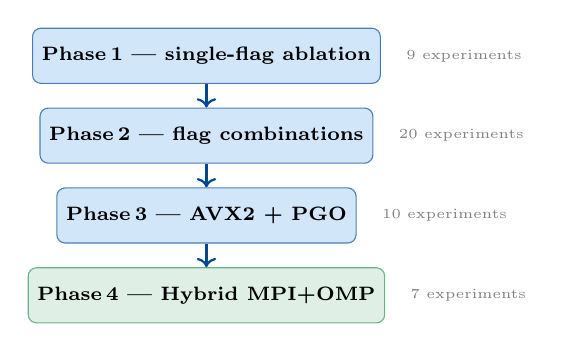
\begin{tikzpicture}[node distance=0.35cm]
        \node[phasebox] (p1) {Phase\,1 — single-flag ablation};
        \node[phasebox, below=0.3cm of p1] (p2) {Phase\,2 — flag combinations};
        \node[phasebox, below=0.3cm of p2] (p3) {Phase\,3 — AVX2 + PGO};
        \node[phasebox, below=0.3cm of p3,
              draw=w3grn!70, fill=w3grn!15] (p4) {Phase\,4 — Hybrid MPI+OMP};
        \draw[->, thick, metnb] (p1) -- (p2);
        \draw[->, thick, metnb] (p2) -- (p3);
        \draw[->, thick, metnb] (p3) -- (p4);
        \node[right=0.2cm of p1, font=\tiny, color=gray] {9 experiments};
        \node[right=0.2cm of p2, font=\tiny, color=gray] {20 experiments};
        \node[right=0.2cm of p3, font=\tiny, color=gray] {10 experiments};
        \node[right=0.2cm of p4, font=\tiny, color=gray] {7 experiments};
      \end{tikzpicture}

      \vspace{0.4em}
      \small
      One variable changed per experiment.\\
      Results logged to \texttt{benchmark\_summary.csv}.
    \end{column}
  \end{columns}
\end{frame}

% ------------------------------------------------------------------
\begin{frame}[shrink=12]{Phase 1 --- single-flag compiler ablation}

  \vspace{-0.3em}
  \begin{center}
  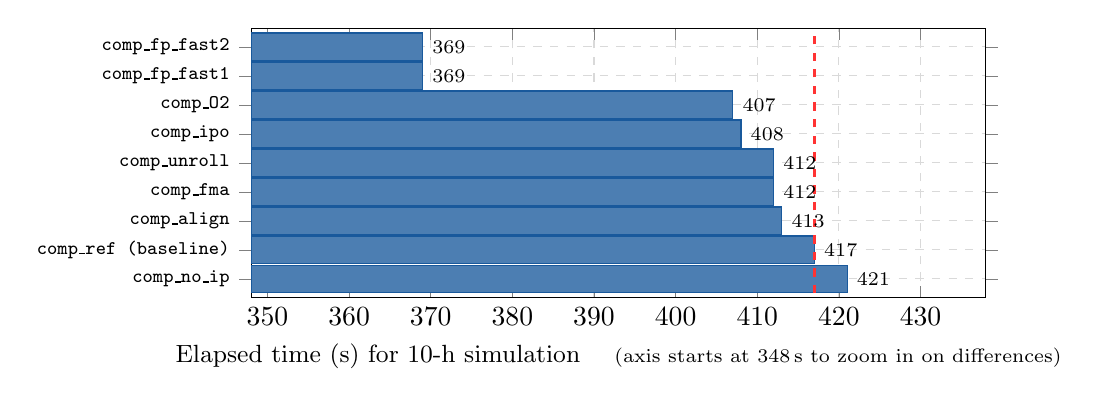
\begin{tikzpicture}
  \begin{axis}[
    xbar,
    width  = 0.90\textwidth,
    height = 5.0cm,
    bar width = 0.35cm,
    xmin = 348, xmax = 438,
    xlabel = {Elapsed time (s) for 10-h simulation
              \quad{\normalfont\scriptsize(axis starts at 348\,s to zoom in on differences)}},
    xlabel style = {font=\small},
    ytick = {1,2,3,4,5,6,7,8,9},
    yticklabels = {
      {comp\_no\_ip},
      {comp\_ref (baseline)},
      {comp\_align},
      {comp\_fma},
      {comp\_unroll},
      {comp\_ipo},
      {comp\_O2},
      {comp\_fp\_fast1},
      {comp\_fp\_fast2}
    },
    yticklabel style = {font=\scriptsize\ttfamily},
    enlarge y limits  = 0.08,
    nodes near coords,
    nodes near coords align = {horizontal},
    every node near coord/.append style = {font=\scriptsize},
    grid = major,
    grid style = {dashed, gray!30},
  ]
    \addplot[fill=metnb!70, draw=metnb!90] coordinates {
      (421,1)(417,2)(413,3)(412,4)(412,5)(408,6)(407,7)(369,8)(369,9)
    };
    % red baseline line at 417 s
    \draw[red!80, dashed, thick]
      (axis cs:417,0.5) -- (axis cs:417,9.5);
  \end{axis}
  \end{tikzpicture}
  \end{center}

  \vspace{-0.3em}
  \small
  \alert{Best single flag:}
  \texttt{-fp-model fast=2} $\Rightarrow$ \textbf{369\,s}
  \quad($-11.5$\,\% vs 417\,s baseline).
  \quad\texttt{-ipo}, \texttt{-unroll}, \texttt{-fma}: individually $<\!2$\,\%.
\end{frame}

% ------------------------------------------------------------------
\begin{frame}[shrink=12]{The \texttt{-xHost} pitfall on AMD EPYC}

  \begin{columns}[T]
    \begin{column}{0.54\textwidth}
      \texttt{-xHost} instructs the Intel compiler to generate code for the
      \emph{highest ISA supported} by the build machine.

      \vspace{0.5em}
      \textbf{On Intel CPUs:} works correctly --- enables AVX-512 or AVX2.

      \vspace{0.4em}
      \textbf{On AMD EPYC Zen\,4:}
      \begin{itemize}
        \item Intel's CPUID probe detects ``not genuine Intel''
        \item Dispatch logic \textbf{silently} falls back to SSE2 safe path
              (128-bit registers instead of 256-bit)
        \item All compute loops run at half the natural vector width
        \item \alert{Result: 1\,188\,s --- $\times$2.8 slower than the 417\,s baseline}
      \end{itemize}

      \vspace{0.3em}
      \begin{alertblock}{Rule for AMD hardware}
        Always use \texttt{-mavx2 -mfma} (explicit ISA targeting).\\
        Never use \texttt{-xHost} or \texttt{-x\textit{ISA}} flags.
      \end{alertblock}
    \end{column}

    \begin{column}{0.42\textwidth}
      \begin{center}
      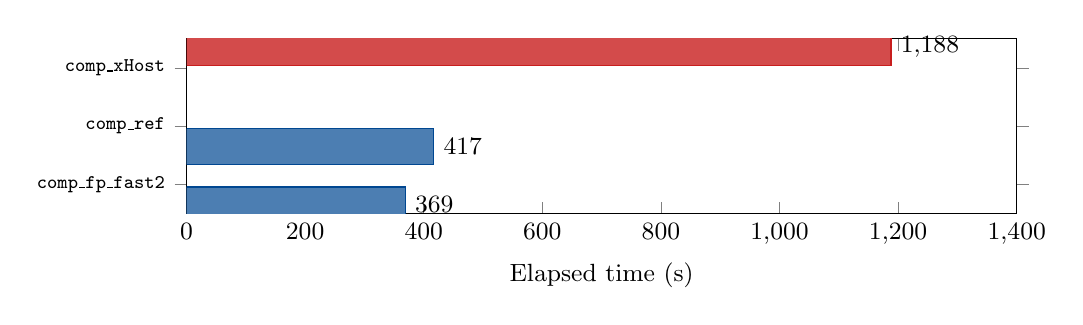
\begin{tikzpicture}
      \begin{axis}[
        xbar,
        width  = \textwidth,
        height = 3.8cm,
        bar width = 0.45cm,
        xmin = 0, xmax = 1400,
        xlabel = {Elapsed time (s)},
        xlabel style = {font=\small},
        ytick = {1,2,3},
        yticklabels = {
          {comp\_fp\_fast2},
          {comp\_ref},
          {comp\_xHost}
        },
        yticklabel style = {font=\scriptsize\ttfamily},
        nodes near coords,
        every node near coord/.append style = {font=\small\bfseries},
        enlarge y limits = 0.25,
        tick label style = {font=\small},
      ]
        \addplot[fill=metnb!70, draw=metnb] coordinates {
          (369,1)(417,2)
        };
        \addplot[fill=w3red!80, draw=w3red] coordinates {
          (1188,3)
        };
      \end{axis}
      \end{tikzpicture}
      \end{center}
      \vspace{2pt}
      \small\centering
      \textcolor{w3red}{\textbf{+185\,\%}} slowdown from a single flag.\\
      Worst result of all 46 experiments.
    \end{column}
  \end{columns}
\end{frame}

% ------------------------------------------------------------------
\begin{frame}[shrink=8]{Phase 2 --- multi-flag combinations}

  Building on the Phase\,1 winner (\texttt{-fp-model fast=2}):

  \vspace{0.2em}
  \begin{center}
  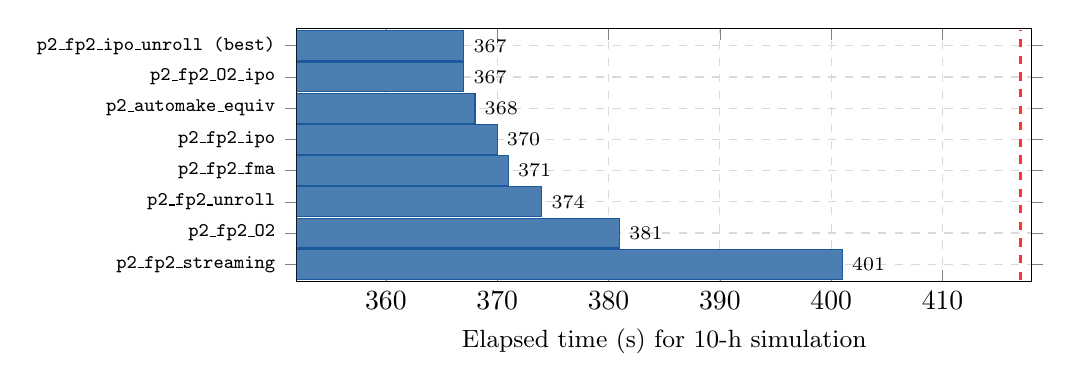
\begin{tikzpicture}
  \begin{axis}[
    xbar,
    width  = 0.90\textwidth,
    height = 4.8cm,
    bar width = 0.38cm,
    xmin = 352, xmax = 418,
    xlabel = {Elapsed time (s) for 10-h simulation},
    xlabel style = {font=\small},
    ytick = {1,2,3,4,5,6,7,8},
    yticklabels = {
      {p2\_fp2\_streaming},
      {p2\_fp2\_O2},
      {p2\_fp2\_unroll},
      {p2\_fp2\_fma},
      {p2\_fp2\_ipo},
      {p2\_automake\_equiv},
      {p2\_fp2\_O2\_ipo},
      {p2\_fp2\_ipo\_unroll (best)}
    },
    yticklabel style = {font=\scriptsize\ttfamily},
    enlarge y limits  = 0.08,
    nodes near coords,
    nodes near coords align = {horizontal},
    every node near coord/.append style = {font=\scriptsize},
    grid = major,
    grid style = {dashed, gray!30},
  ]
    \addplot[fill=metnb!70, draw=metnb!90] coordinates {
      (401,1)(381,2)(374,3)(371,4)(370,5)(368,6)(367,7)(367,8)
    };
    \draw[red!80, dashed, thick]
      (axis cs:417,0.5) -- (axis cs:417,8.5);
    \node[red!80, font=\scriptsize, anchor=west]
      at (axis cs:418,1) {417\,s};
  \end{axis}
  \end{tikzpicture}
  \end{center}

  \vspace{-0.2em}
  \small
  \alert{Best:} \texttt{-fp-model fast=2 -ipo -unroll-aggressive}
  $\Rightarrow$ \textbf{367\,s} ($-12.0$\,\%).
  \quad Note: automake-equivalent flags give similar performance (368\,s).
\end{frame}

% ------------------------------------------------------------------
\begin{frame}[shrink=12]{Phase 3 --- AVX2 vectorisation + Profile-Guided Optimisation}

  \begin{columns}[T]
    \begin{column}{0.55\textwidth}
      \textbf{Stage A: explicit AVX2 targeting}
      \begin{itemize}
        \item Add \texttt{-mavx2 -mfma -fno-alias} to Phase\,2 best build
        \item Forces 256-bit FP lanes; default SSE2 only uses 128-bit
        \item \texttt{p3\_fp2\_ipo\_unroll\_avx2\_nd}: \textbf{355\,s}
              ($-14.9$\,\%)
      \end{itemize}

      \vspace{0.5em}
      \textbf{Stage B: Profile-Guided Optimisation (PGO)}
      \begin{enumerate}
        \item Compile with \texttt{-prof-gen} (instrumented binary)
        \item Run a representative 1-hour simulation (profile collection)
        \item Recompile with \texttt{-prof-use} (apply profile data)
      \end{enumerate}
      PGO improves: hot-path inlining decisions, branch layout,
      and loop unroll factors tailored to actual WW3 execution traces.

      \vspace{0.4em}
      \texttt{p3\_pgo\_avx2\_nd}: \textbf{326\,s} ($-21.8$\,\%)
    \end{column}

    \begin{column}{0.42\textwidth}
      \begin{center}
      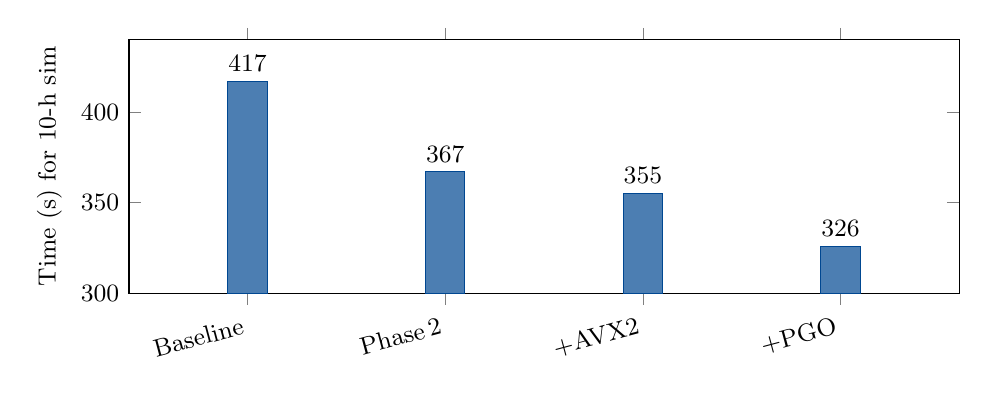
\begin{tikzpicture}
      \begin{axis}[
        ybar,
        width  = \textwidth,
        height = 4.8cm,
        bar width = 0.50cm,
        ymin = 300, ymax = 440,
        ylabel = {Time (s) for 10-h sim},
        ylabel style = {font=\small},
        xtick = data,
        xticklabels = {Baseline, Phase\,2, +AVX2, +PGO},
        xticklabel style = {font=\small, rotate=15, anchor=north east},
        tick label style = {font=\small},
        nodes near coords,
        every node near coord/.append style = {font=\small\bfseries},
        enlarge x limits = 0.2,
        yticklabel style = {font=\small},
      ]
        \addplot[fill=metnb!70, draw=metnb] coordinates {
          (1,417)(2,367)(3,355)(4,326)
        };
      \end{axis}
      \end{tikzpicture}
      \end{center}
      \small\centering
      Cumulative gains: from 417\,s to 326\,s\\
      $= -21.8$\,\% without touching the job layout.
    \end{column}
  \end{columns}
\end{frame}

% ------------------------------------------------------------------
\begin{frame}[shrink=18]{Phase 4 --- Hybrid MPI + OpenMP}

  \begin{columns}[T]
    \begin{column}{0.52\textwidth}
      Starting from the PGO binary ($\sim$326\,s), OpenMP hybrid modes
      were added via the \texttt{OMPH}+\texttt{OMPG} switch pair.

      \vspace{0.5em}
      \textbf{Variant A} (48 ranks/node $\times$ 3 CPUs/rank):
      \begin{itemize}
        \item 768 total ranks; 2 OMP compute threads + 1 async-MPI thread
        \item \textcolor{w3red}{Did not complete} --- instability in the
              3-CPU async configuration
      \end{itemize}

      \vspace{0.4em}
      \textbf{Variant B} (60 ranks/node $\times$ 2 CPUs/rank, async off):
      \begin{itemize}
        \item Same 1\,920 CPUs as the MPI-only baseline
        \item \texttt{I\_MPI\_ASYNC\_PROGRESS=0} --- no async thread
        \item Both CPUs run OMP compute threads
        \item \texttt{OMP\_NUM\_THREADS=2}
        \item \alert{Result: \textbf{290\,s} ($-30.5$\,\% vs 417\,s)}
      \end{itemize}

      \vspace{0.3em}
      Throughput: \textbf{5.17 simulated days / wall-clock hour}

      \vspace{0.3em}
      \begin{exampleblock}{Production scaling}
        \small
        When applied to a full storm case, this OMPH config
        ran \textbf{7 simulation days in 1 wall-clock hour}.
      \end{exampleblock}
    \end{column}

    \begin{column}{0.44\textwidth}
      \begin{center}
      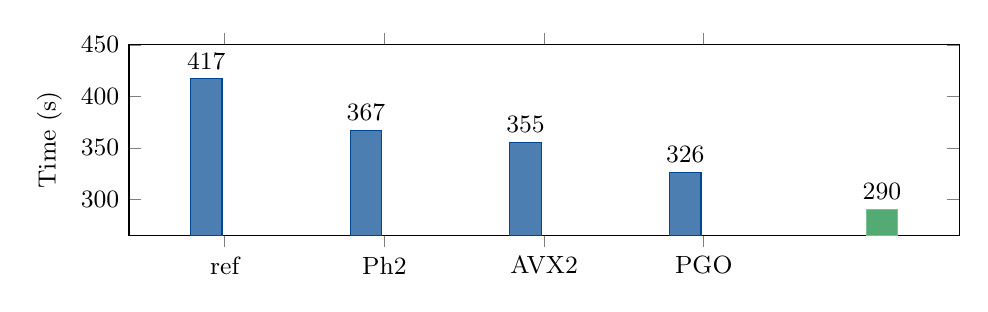
\begin{tikzpicture}
      \begin{axis}[
        ybar,
        width  = \textwidth,
        height = 4.0cm,
        bar width = 0.40cm,
        ymin = 265, ymax = 450,
        ylabel = {Time (s)},
        ylabel style = {font=\small},
        xtick = data,
        xticklabels = {ref, Ph2, AVX2, PGO, OMPH},
        xticklabel style = {font=\small},
        tick label style = {font=\small},
        nodes near coords,
        every node near coord/.append style = {font=\small\bfseries},
        enlarge x limits = 0.15,
        yticklabel style = {font=\small},
      ]
        \addplot[fill=metnb!70, draw=metnb] coordinates {
          (1,417)(2,367)(3,355)(4,326)
        };
        \addplot[fill=w3grn!80, draw=w3grn!60] coordinates {
          (5,290)
        };
      \end{axis}
      \end{tikzpicture}
      \end{center}
      \small\centering
      \textcolor{w3grn}{\textbf{290\,s}} = best result.\\
      Final 36\,s gain comes entirely from
      converting the idle async thread into an OMP compute thread.
    \end{column}
  \end{columns}
\end{frame}

% ------------------------------------------------------------------
\begin{frame}[shrink=10]{Summary --- end-to-end improvement}

  \begin{columns}[T]
    \begin{column}{0.52\textwidth}
      \begin{tabular}{llrr}
        \toprule
        Stage & Experiment & Time (s) & Gain \\
        \midrule
        Baseline  & \texttt{comp\_ref}        & 417 & ---          \\
        Phase\,2  & \texttt{fp2+ipo+unroll}   & 367 & $-12.0$\,\%  \\
        Phase\,3A & \texttt{+avx2}            & 355 & $-14.9$\,\%  \\
        Phase\,3B & \texttt{+pgo}             & 326 & $-21.8$\,\%  \\
        Phase\,4  & \texttt{+omph (varB)}     & \textbf{290} & \textbf{$-30.5$\,\%} \\
        \bottomrule
      \end{tabular}

      \vspace{0.7em}
      \textbf{Total reduction:} 127\,s per 10-hour simulation.
    \end{column}

    \begin{column}{0.44\textwidth}
      \begin{center}
      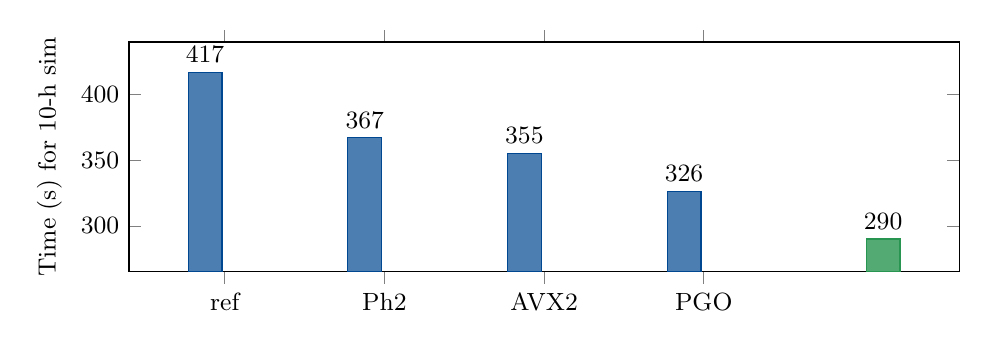
\begin{tikzpicture}
      \begin{axis}[
        ybar,
        width  = \textwidth,
        height = 4.5cm,
        bar width = 0.43cm,
        ymin = 265, ymax = 440,
        ylabel = {Time (s) for 10-h sim},
        ylabel style = {font=\small},
        xtick = data,
        xticklabels = {ref, Ph2, AVX2, PGO, OMPH},
        xticklabel style = {font=\small},
        tick label style = {font=\small},
        nodes near coords,
        every node near coord/.append style = {font=\small\bfseries},
        enlarge x limits = 0.15,
        yticklabel style = {font=\small},
      ]
        \addplot[fill=metnb!70, draw=metnb] coordinates {
          (1,417)(2,367)(3,355)(4,326)
        };
        \addplot[fill=w3grn!80, draw=w3grn] coordinates {
          (5,290)
        };
      \end{axis}
      \end{tikzpicture}
      \end{center}
    \end{column}
  \end{columns}
\end{frame}

% ------------------------------------------------------------------
\begin{frame}{Take-home messages}

  \begin{enumerate}\setlength\itemsep{0.2em}
    \item \textbf{Measure on your actual machine.}
          Results for Intel CPUs do not transfer to AMD (or vice versa).

    \item \textbf{Start with model-side levers} (grid, I/O, output fields)
          --- they require no recompilation and can give 10--20\,\%.

    \item \textbf{Floating-point model beats loop flags.}
          \texttt{-fp-model fast=2} gave $11.5$\,\%; aggressive unrolling alone
          gave $<\!2$\,\%.

    \item \textbf{Explicit SIMD targeting is non-negotiable on AMD EPYC.}
          \texttt{-xHost} caused a $\times\!2.8$ slowdown.
          Use \texttt{-mavx2 -mfma}.

    \item \textbf{PGO is worth the effort.}
          Additional $7$\,\% on top of AVX2 with no model change.

    \item \textbf{Convert the async-MPI thread into a compute thread.}
          Setting \texttt{I\_MPI\_ASYNC\_PROGRESS=0} + \texttt{OMP\_NUM\_THREADS=2}
          unlocked the final 10\,\%.

    \item \textbf{One variable at a time.}
          Phased ablation gives interpretable, reproducible results.
  \end{enumerate}
\end{frame}

% ------------------------------------------------------------------
\begin{frame}[standout]
  \begin{center}
    {\Huge Thank you!}\\[1.2em]
    {\Large Questions?}
  \end{center}
  \vspace{0.6em}
  \begin{center}
    \small
    Results: \texttt{benchmark\_summary.csv}\\
    Scripts: \texttt{benchmarking/run\_*.sh}\\
    Recipe: \texttt{docs/recipe\_benchmarking.md}\\[0.5em]
    \normalsize
    \textbf{Repository:}\\[0.2em]
    \texttt{\scriptsize https://github.com/lenny-frno/WW3\_calibration/tree/main}\\[0.8em]
    
\includegraphics[height=0.8cm]{met-rgb-horisontal-eng.jpg}
  \end{center}
\end{frame}

% ==========================================================================
\end{document}
% ==========================================================================
